\section{Stereoscopy}
\label{sec:backgr:stereo}

Our brain is able to understand depth by leveraging the fact that we have two eyes in slightly different positions.
This mechanism is called stereoscopy, and it can be used by a computer vision system, provided that it has two or more cameras.

\begin{figure}
	\centerline{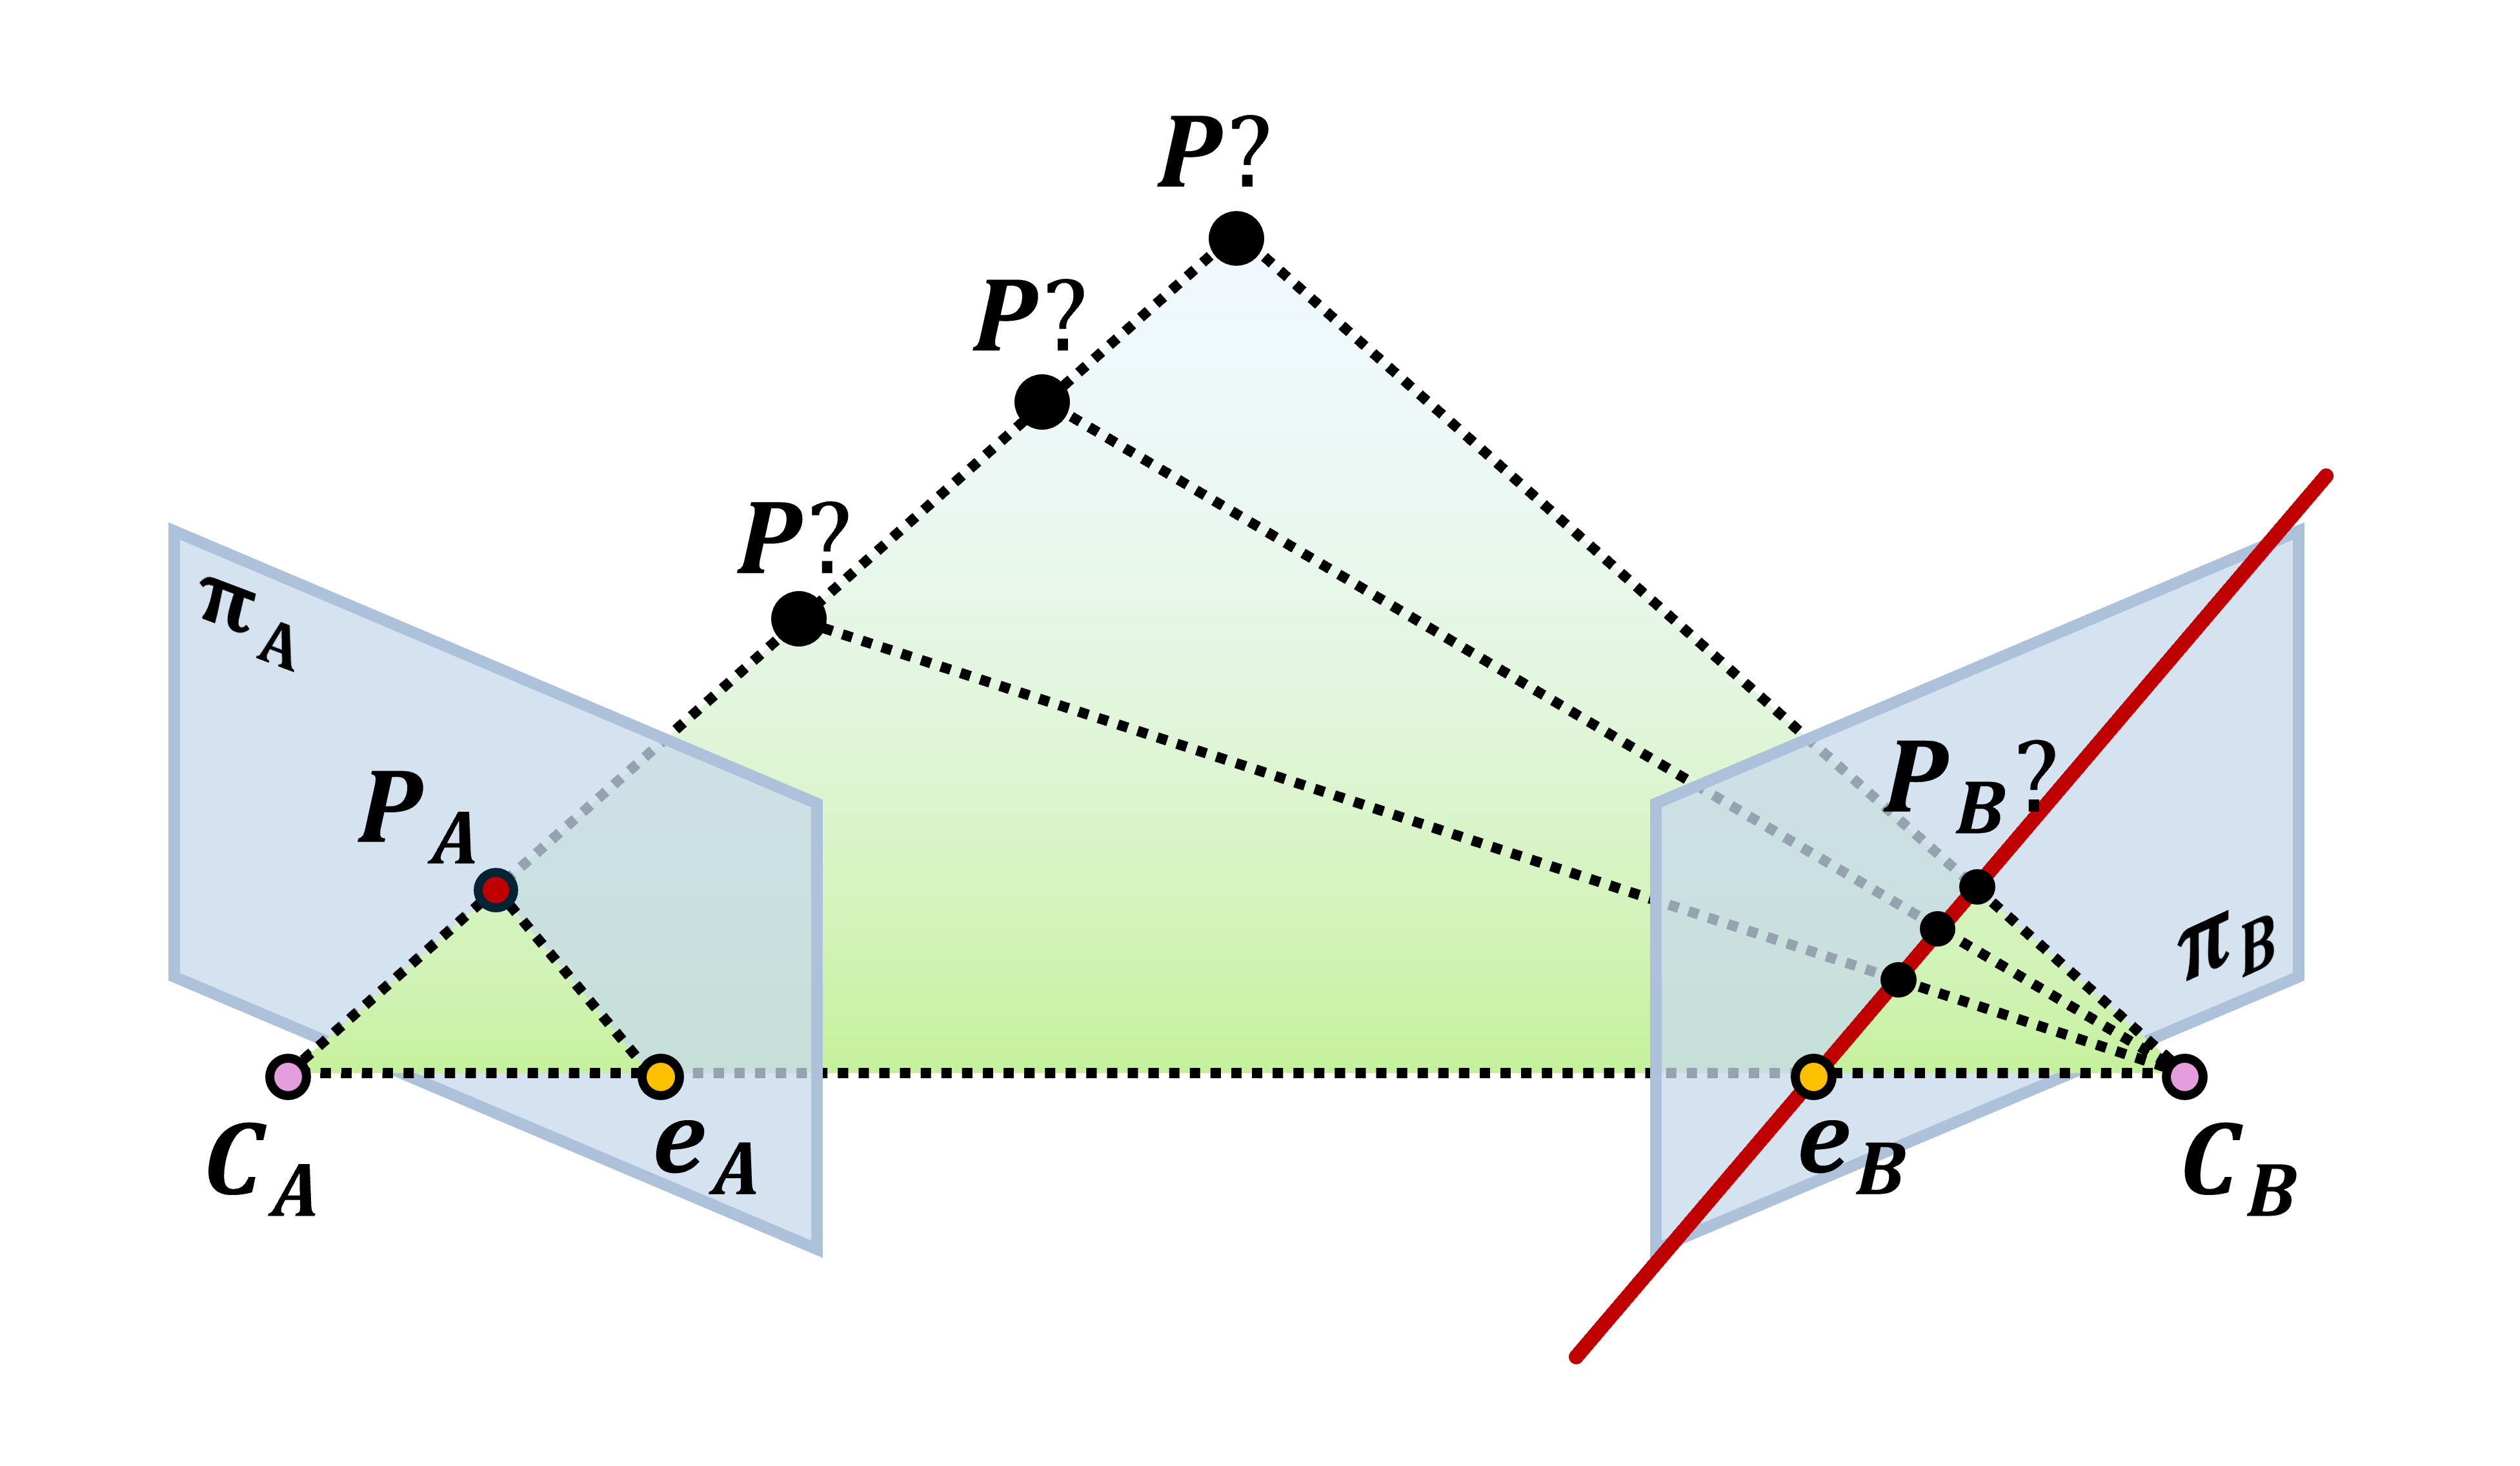
\includegraphics[width=0.8\textwidth]{images/epipolarity.png}}
	\caption{\centering Reprojecting a point from 2D to 3D: it could be anywhere on a specific line}
	\label{fig:epipolarity}
\end{figure}

\subsection{Depth estimation}

Consider a camera $A$, with center of projection $C_A$ and image plane $\pi_A$ (left in figure~\ref{fig:epipolarity}).
If a 3D point $P$ is seen by the camera, in the image plane it will be $P_A = \pi_A \cap \overline{PC_A}$.
From a single camera, it is impossible to reconstruct $P$ from $P_A$: there would be infinitely many possible $P$s, all the points that lie on the extension of $\overline{P_AC_A}$.

If another camera $B$ is available (right in figure~\ref{fig:epipolarity}), and the same point $P$ is projected as $P_B$, then a new information is added: that $P$ will lie on the extension of $\overline{P_BC_B}$.
By intersecting these lines, it is ideally possible to reconstruct the original 3D position of $P$.

In order to do so, the relative position of the cameras needs to be known: all calibration parameters are required.
In particular, the function \texttt{triangulatePoints} from \texttt{OpenCV} is able to reconstruct the 3D positions given the 2D matched observations, the intrinsic and distortion parameters of the two cameras, and the extrinsic matrix of the couple.

\subsection{Epilines}
\label{sec:backgr:stereo:epilines}

As stated before, the point $P_A$ could correspond to a full line of 3D points.
When seen by camera $B$ (with a different point of view), this line translates to a 2D line in $\pi_B$ (red in figure~\ref{fig:epipolarity}).
This line is called \textbf{epiline}.

Different points $P_A$ will correspond to different epilines, which however all pass by the \textbf{epipoint} $e_B$.
The epipoint is defined as $e_B = \pi_B \cap \overline{C_AC_B}$.

\subsubsection{Computing the epiline equation}

As explained in the previous section, the essential matrix $E$ is such that $P_B \cdot E \cdot P_A^T = 0$, which is called the \textbf{epipolar constraint}.
If $P_B$ is a generic point on the image, it can be described as $P_B = \rowvecthree{x}{y}{1}$.
The result of $E \cdot P_A^T$ is a $3\times 1$ vector, that can be written without loss of generality as $\rowvecthree{a}{b}{c}^T$.
When all this knowledge is substituted into the epipolar constraint, we obtain the following:
$$ \rowvecthree{x}{y}{1} \cdot E \cdot P_A^T = 0\\ $$
$$ \rowvecthree{x}{y}{1} \cdot \colvecthree{a}{b}{c} = 0\\ $$
$$ ax + by + c = 0 $$
which is the equation of the epiline in $B$'s frame.
% When this information is substituted into the epipolar constraint, the result of the product becomes the equation $ax + by + c = 0$, where $a$, $b$ and $c$ come from $E \cdot P_A^T$.
% Therefore, the epipolar line is 

\subsection{3D matching}

For estimating the depth, \texttt{triangulatePoints} needs matched point.
That is, the $i{-}th$ point provided by camera $A$ and the $i{-}th$ point provided by camera $B$ must be the two projections of the same 3D point.
To perform this matching, traditional stereoscopy follows this procedure:
\begin{enumerate}
	\itemsep 0em
	\item Choose a point in the main image;
	\item Compute the equation of the corresponding epiline;
	\item Consider a patch around the original point;
	\item For each point on the epiline (in the second image), compute the similarity of a patch centered in that point with the original patch;
	\item Select the most similar point as the match;
	\item Compute the 3D coordinate of the point from the obtained match.
\end{enumerate}
